% !TEX root = mainthesis.tex

%Chapter 4


\renewcommand{\thechapter}{4}


\chapter{Making BECs in the Rubidium Lithium apparatus}

All the experiments presented in this thesis were performed at the Rubidium-Lithium (RbLi) apparatus at the University of Maryland. The experiment was designed to produce mixtures of quantum degenerate gases of bosons and fermions. The original plan was abandoned because the cross-species scattering length was found to be repulsive and small ($a_s\approx20\,a_B)$~\cite{silber_quantum-degenerate_2005} and the nearest heteronuclear $s$-wave Feshbach resonance was measured to occur at the unexpectedly large magnetic field of $\unit[1066]{G}$~\cite{deh_feshbach_2008} and therefore all our experiments were performed using only $\Rb87$.

The RbLi apparatus is scheduled to be shut down and the construction of a new dual-species apparatus for $\Rb87$ and K$^{39}$ is underway. The RbLi apparatus has been thoroughly described in \cite{CampbellThesis,PriceThesis}. Here I only give a brief overview of the apparatus. Additionally I discuss new elements that have been added to the setup and changes that have been implemented and were not reported in previous thesis.  

This Chapter is divided into three sections. In Section~\ref{sec:RbLi_overview} I give a brief overview of the RbLi apparatus and describe its basic capabilities. In Section~\ref{sec:making-becs} I describe the experimental sequence used to produce BECs. Finally in Section~\ref{sec:RbLi_upgrades} I describe changes and to the RbLi apparatus that have not been reported on previous theses. 

\section{Overview of the RbLi apparatus}
\label{sec:RbLi_overview}

In this section I briefly describe the setup of and basic capabilities of the RbLi apparatus. Figure~\ref{fig:RbLi} shows the main optical table where atoms are cooled to degeneracy. The vacuum system can be divided into three regions: an oven Region where Rb and Li atoms are heated up, a Zeeman slower that acts as a differential pumping stage and an ultra-high vacuum region with a glass cell where all the experiments are performed.

\begin{figure*}[htb]
\begin{center}
\includegraphics[]{Figures/Chapter4/RbLi_basic.pdf}
\caption[The RbLi vacuum system]{$\Rb87$ level structure (not to scale). {\bf a.} Ground and first excited state electronic configuration of $\Rb87$ given by the $\{n,\mathbf{L}\}$ quantum numbers. {\bf b.} The interaction between the orbital angular momentum and the spin of the electron leads to the fine splitting of orbitals with $L>0$. The splitting of the $5^2P$ line gives rise to the D1 and D2 lines. {\bf c.} The interaction between the total angular momentum and the nuclear spin causes the fine structure levels to split further into states characterized by the quantum number $F$.}
\label{fig:RbLi}
\end{center}
\end{figure*}

 We can detect atoms using two different imaging systems. The first one is used primarily for diagnostics and it images the $yz$ plane of the atoms from the $+\ex$ side of the glass cell. The second system looks at the $xy$ plane from bellow the glass cell and is the main system used for data acquisition (see Figure~\ref{fig:RbLi_diagram}). 

\subsection{Laser systems}

We use a total of three lasers to perform laser cooling and imaging of atoms: a cooling laser that addresses the $F=2\rightarrow F'=3$ transition, a repump laser that takes atoms that have decayed into the $F=1$ state back to $F=2$ and a master laser that provides a frequency reference for both lasers. The frequency of master laser is locked using saturation absorption spectroscopy to the $F=3\rightarrow F'=3$ and $F=3\rightarrow F'=4$ crossover of the D2 line of $^{85}$Rb. 

We have two additional lasers that are used to generate potentials for the atoms. The first one is a $\unit[30]{W}$ $\unit[1064]{nm}$ \noted{IPG Photonics} laser that we use to make a cross dipole trap for the atoms. The two dipole beams come from the zeroth and first order of an acusto optic modulator (AOM) and the beams propagate along the $\ex+\ey$ and $\ex-\ey$ direction. The other laser system is a Ti:Saphire laser used to generate Raman transitions and will be described in more detail in Section~\ref{sec:Raman_laser}. Figure~\ref{fig:RbLi_diagram} shows a simplified diagram with a bird's-eye view and a side view of the apparatus that show all the lasers that are used for cooling, trapping, Raman coupling and imaging.

\begin{figure*}[!t]
\begin{center}
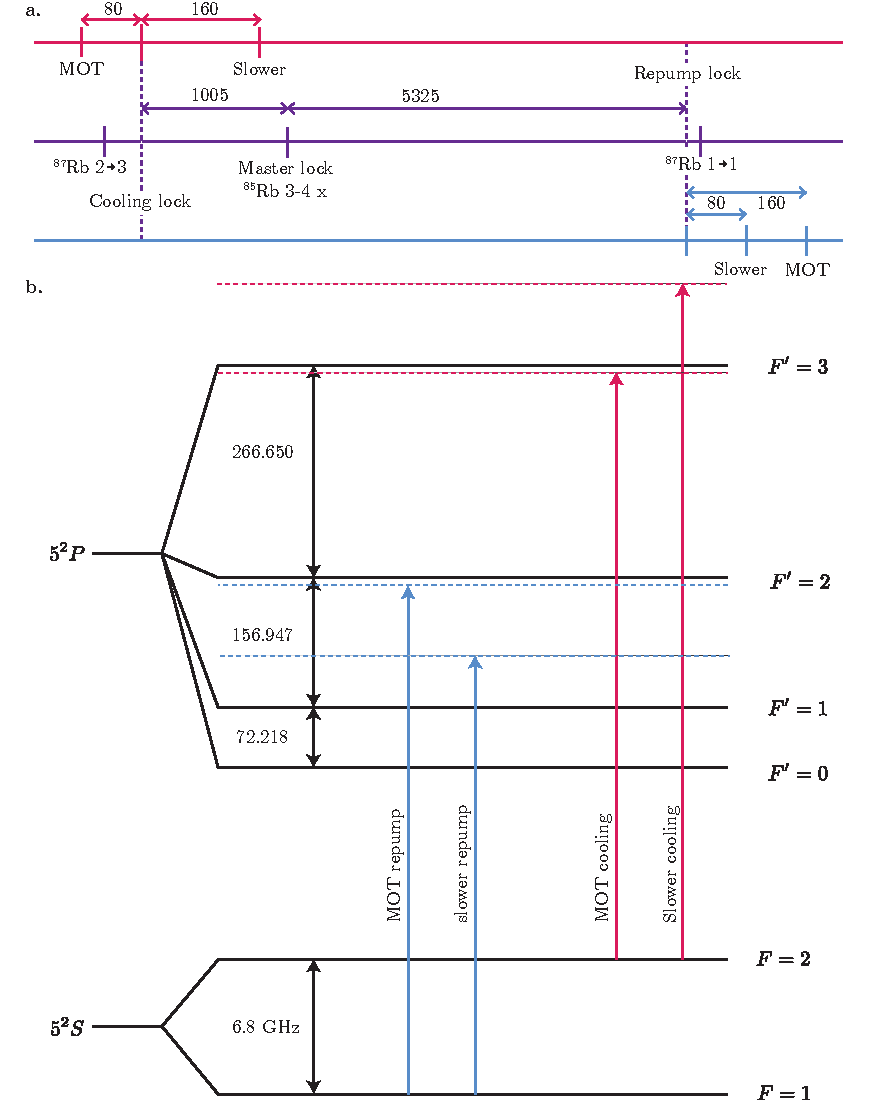
\includegraphics[]{Figures/Chapter4/laser_frequencies.pdf}
\caption[Laser cooling frequencies]{{\bf a.}Cooling and repump frequencies relative to the master laser lock. {\bf b.} Cooling and repump frequencies relative to the $\Rb87$ D2 line transitions.}
\label{fig:laser_frequencies}
\end{center}
\end{figure*}

\begin{figure*}[!h]
\begin{center}
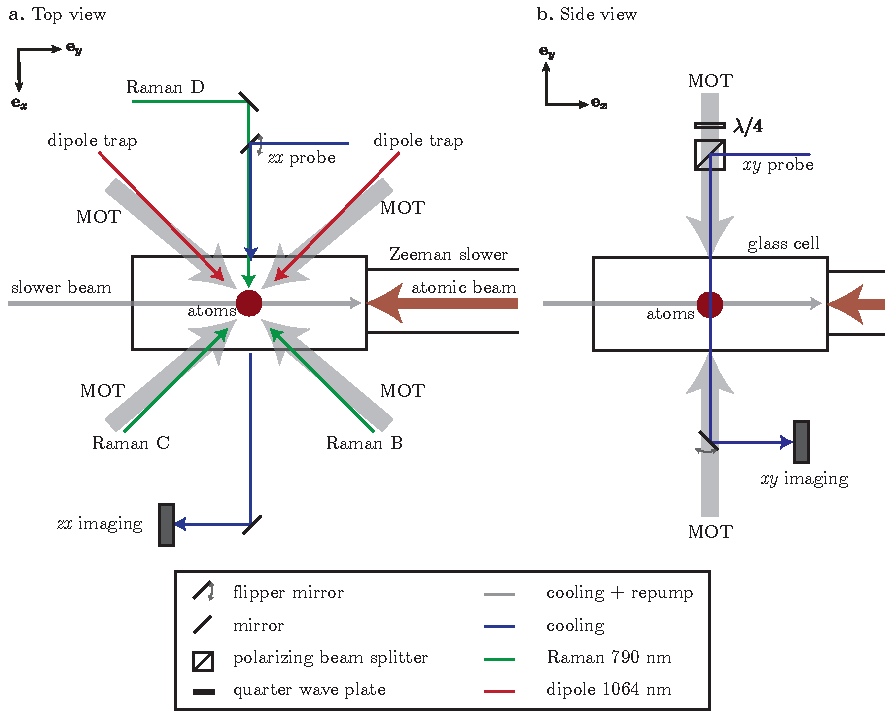
\includegraphics[]{Figures/Chapter4/RbLi_diagram.pdf}
\caption[Laser cooling frequencies]{{\bf a.}Cooling and repump frequencies relative to the master laser lock. {\bf b.} Cooling and repump frequencies relative to the $\Rb87$ D2 line transitions.}
\label{fig:RbLi_diagram}
\end{center}
\end{figure*}

\subsection{Magnetic field control}

The precise control of magnetic fields is essential during the multiple stages in our experimental sequence. We use multiple coils in our experiment as is illustrated in Figure~\ref{fig:bias_coils}.   Three pairs of Helmholtz coils in the vicinity of the glass cell generate bias magnetic fields along $\ex$, $\ey$ and $\ez$.  Once BECs are produced we typically use bias fields along $\ez$ to change the Zeeman energy of the different $m_F$ states. One pair of anti-Helmholtz coils generates a strong quadrupole magnetic field along $\ez$ that is used in the MOT, for magnetic trapping and for Stern-Gerlach in time of flight. An additional set of coils arranged in a `clover leaf' pattern generates small gradients along $\ez$, $\ex+\ey$ and $\ez-\ey$ which allow us to cancel stray magnetic gradients at the location of the atoms.  

The experiment also has the capability of producing oscillatory magnetic fields. A set of coils on a printed circuit board (PCB) produce linearly polarized radio-frequency (RF) magnetic fields either in the $\ey$ or $\ez$ direction that are used for RF induced evaporation and to drive transitions between $m_F$ states. The setup for producing high-power RF fields will be described in more detail in Section~\ref{sec:high_power_rf_antenna}.

\begin{figure*}[htb]
\begin{center}
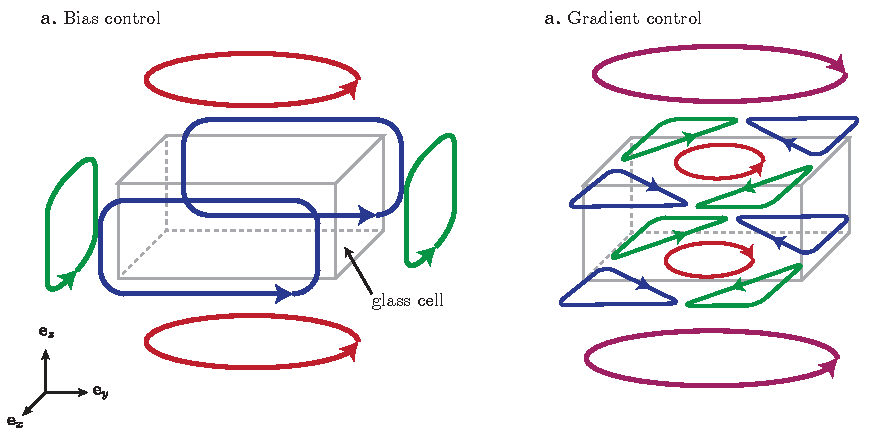
\includegraphics[]{Figures/Chapter4/bias_coils.pdf}
\caption[Magnetic coil geometry in the RbLi apparatus]{Magnetic coil geometry in the RbLi apparatus.{\bf a.} We use three pairs of Helmholtz coils to produce bias fields along $\ex$, $\ey$ and $\ez$. {\bf b.} We have a pair of coils that produce strong quadrupole magnetic fields for the MOT and magnetic trapping. Additionally we have a pair of `clover-leaf' coils to control the gradients along $\ez$.}
\label{fig:bias_coils}
\end{center}
\end{figure*}

\section{Experimental sequence to make BECs}
\label{sec:making-becs}

In this section I list the steps in our experimental sequence that produces $\Rb87$ BECs.

The production of BECs starts in an oven where Rb atoms are heated to $\unit[120]{^{\circ}C}$ to produce an atomic beam. The atoms then travel down a Zeeman slower~\cite{phillips_laser_1982} where they are laser cooled. The slowed down atoms are then captured in a magneto-optical trap (MOT) in a glass cell. For the MOT we apply a $\unit[5.5]{A}$ current to the quadrupole coils corresponding to a $\unit[15.62]{G/cm}$ gradient. The cooling light is blue detuned by $\unit[18]{MHz}~-2\Gamma$ from the $F=2\rightarrow F'=3$ cycling transition and the repump light is $\unit[16]{MHz}$ below the $F=1\rightarrow F'=2$ transition. We typically load the MOT for times between $\unit[1-5]{s}$. In preparation for the molasses stage we do a $\unit[30]{ms}$ decompression stage where we ramp down the gradient to $\unit[10]{G/cm}$ and reduce the repump power. The slower currents and light are turned off before this stage.

The next step is to perform polarization gradient cooling in optical molasses where the polarization gradient from interfering counter propagating lasers further cools the atoms~\cite{lett_observation_1988}. For this we completely switch off the quadrupole coils and adjust the bias fields in all three directions so that they are zero at the atoms. During this stage the repump power is kept low and the frequency of the cooling light is decreased to $\unit[140]{MHz}$ below the MOT values for $\unit[10]{ms}$. We then completely turn off the MOT repump light to allow atoms to decay into the $F=1$ manifold and use some slower repump light to optically pump atoms into the $\ket{F=1,m_f=-1}$ magnetically trappable state for a total of $\unit[1.5]{ms}$.

Once the atoms are succesfully pumped into $\ket{F=1, m_f=-1}$ we capture them in a magnetic trap with a gradient of $\unit[62]{G/cm}$ and compress them by increasing the current in the coils until we reach a gradient of $\unit[160]{G/cm}$ in $\unit[300]{ms}$. In the magnetic trap we perform RF induced evaporation by turning on an RF field polarized along $\ey$ with frequency of $\unit[24]{MHz}$, which transfers the hotter atoms at the edges of the trap into the $m_f=0$ state which is not magnetically trappable. We then perform an exponential ramp from the initial frequency to a final frequency of $\unit[4.5]{MHz}$ in $\unit[1]{s}$. 

We then proceed to transfer the atoms from the magnetic trap into a dipole trap. We start by turning on only the `tight' arm of the dipole trap at full power (about $\unit[11]{W}$) and slowly decompressing the quadrupole trap to $\unit[45]{G/cm}$ in $\unit[1.5]{s}$. We then turn on the second `cross' dipole beam in $\unit[1]{s}$; splitting the power so that there the power split between the tight and cross beams is about $70-30\%$. As the cross dipole beam is being turned on we ramp the quadrupole field further down to $\unit[14]{G}[cm]$, slightly above the value necessary for the trap to suspend atoms against gravity. We simultaneously shift the bias field along $\ez$ to align the center of the quadrupole trap to the dipole trap. 

We evaporate the atoms in the dipole trap in two stages. First we exponentially ramp down the power to about $20\%$ of its initial power in $\unit[1.5]{s}$ (time constant $=\unit[0.5]{s}$). Before the final evaporation stage we completely turn off the quadrupole trap in $\unit[1]{s}$. Finally, we perform a second exponential ramp where the power is dropped to about $30\%$ of the intermediate power in $\unit[2]{s}$ (time constant $=\unit[1]{s}$. The slow ramps ensure that there is enough time for the atoms to thermalize as they evaporate.   During the second evaporation stage the atoms reach the critical temperature for Bose-Einstein condensation and we are able to produce BECs with about $4\times10^4$ atoms in the $\ket{F=1, m_f=-1}$ state.
At this point we can prepare different $m_f$ states and set the Zeeman splitting between levels using the techniques described in the following sections. 

\subsection{Adiabatic rapid passage}
\label{sec:arp}

We prepare different $m_f$ states within the $F=1$ manifold using an adiabatic rapid\footnote{Rapid with respect to the spontaneous emission rate of the excited state being coupled.} passage protocol (ARP) which is based on the Landau-Zener model~\cite{zener_non-adiabatic_1932}. The technique relies on preparing dressed states; eigenstates of the atomic Hamiltonian with an oscillatory field magnetic field (typically RF or microwaves for us). To perform ARP with RF we set the frequency of the field $\omega_{\rm{RF}}$ so that it matches the Zeeman splitting between the $m_f=-1$ and $m_f=0$ for a target bias field $B_0\ez$.

We start with atoms in $m_F=-1$ and at a bias field $B_i\approx B_0-\unit[380]{mG}$ ($\delta\approx\unit[30]{kHz}$). We ramp an $\Omega=\unit[20]{kHz}$ RF field and frequency $\sim B_0*0.7$ in $\unit[50]{ms}$, effectively preparing atoms in the ground dressed state shown in Figure~\ref{sec:arp}a. We then sweep the detuning by linearly changing the bias field. As the detuning is changed, the state decomposition of the ground state is modified and as long as the rate of change in detuning is small compared to $\Omega_{\rm{RF}}^2$ (the gap in Figure~\ref{sec:arp}a) the system will adiabatically follow. Finally the RF field is abruptly turned off, projecting the RF eigenstates into the $m_f$ states. In Figure~\ref{sec:arp} we set $\omega_{\rm{RF}}=\unit[23]{MHz}$ and when the Zeeman splitting between $m_F=-1$ and $m_F=0$ is equal to $\omega_{\rm{RF}}$ we observe an equal superposition of both states and if the detuning is swept beyond resonance we can reliably prepare the $m_f=0$ state. In general it is necessary to look at the eigenstates of the three-level RF Hamiltonian
%
\begin{equation}
\hat{H}_{\rm{RF}}=\begin{pmatrix}
-\delta & \Omega_{\rm{RF}}/2 & 0  \\
\Omega_{\rm{RF}}/2 & -\epsilon & \Omega_{\rm{RF}}/2  \\
0 & \Omega_{\rm{RF}}/2 & \delta  
\end{pmatrix},
\end{equation}
%
but for large quadratic Zeeman shifts as is usually the case in our experiments we can only look at an effective two-level system.

In order to keep the bias fields as stable as possible we also synchronize the timing of our experiments to the $\unit[60]{Hz}$ line; this step is performed in different stages of the experiment but perhaps were we have noted it has the biggest impact is right before ARP. For additional magnetic field control and stabilization we use a technique using microwave assisted partial transfer absorption imaging described in the following section. 

\begin{figure*}[htb]
\begin{center}
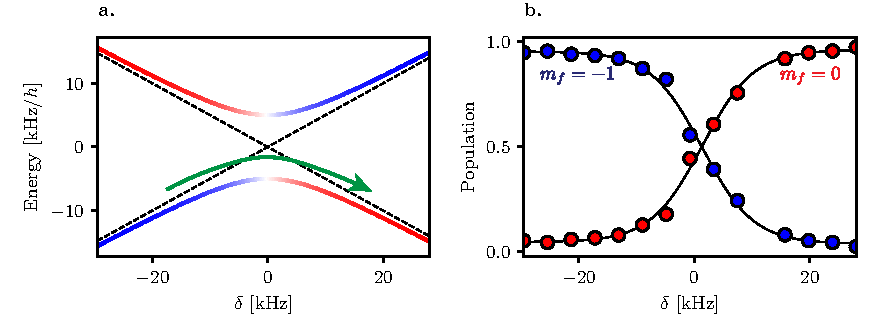
\includegraphics[]{Figures/Chapter3/arp_anotated.pdf}
\caption[Adiabatic rapid passage]{{\bf a.} Eigenenergies and eigenstate decomposition of an RF dressed Hamiltonian (Equation~\ref{eq:h_rwa}) with $\Omega=10$as a function of detuning. The eigenstates are linear combinations of $m_f=-1$ and $m_f=0$ (red and blue respectively). {\bf b.} Population in the $m_f$ sates for different values of detuning}
\label{fig:arp}
\end{center}
\end{figure*}

\subsection{Magnetic field stabilization with microwave assisted partial transfer absorption imaging}
\label{sec:ptai}

Our experiments are very sensitive to changes in the environmental magnetic field. In the past we used flux gate sensors (\noted{Stefan-Mayer} model \noted{FL1-100 f}) in the apparatus to feedback and stabilize the magnetic field (see~\cite{PriceThesis}. This sensors are a useful tool, however due to space constrains we were not able to measure the fields close to the atoms and additionally the range of magnetic fields that they operate at is small (only $\unit[1]{G}$, we typically operate at $>\unit[10]{G}$). We built a $\unit[6.8]{GHz}$ microwave system so that we could use the atoms themselves as sensors of magnetic field.

The method relies in transferring a small fraction of atoms into the $F=2$ manifold where they can be imaged without the use of repump light and therefore minimally disturbing the remaining atoms in $F=1$. We apply two microwave pulses with frequency $\omega_0$ for a total time $\tau$ and coupling strength $\Omega_0\ll 1/\tau$, each detuned by $\delta_{\pm}=\pm1/(2\tau)$ from the target resonance frequency. We image the transferred atoms following each pulse using absorption imaging and from the measured densities we calculate the imbalance
%
\begin{equation}
 	n_{\rm{imb}}=\frac{n(\delta_+)-n(\delta_-)}{n(\delta_+)+n(\delta_-)}
 \end{equation} 
%
which gives us a signal that is both insensitive to fluctuations in the number of atoms and linearly sensitive to changes in magnetic field\footnote{A single pulse on resonance is quadratically sensitive to detuning (see Equation~\ref{eq:Rabi_oscillations})}. We use this error signal both to monitor the magnetic field before performing experiments and cancel longterm drifts in the field. In most cases, we chose the states $\ket{F=1, m_f=-1}$ and $\ket{F=2, mf=-2}$ as their relative energies are the most sensitive to changes in magnetic field. Figure~\ref{fig:uwave_lock}a shows the transfered atoms by each microwave pulse for different values of bias magnetic field and Figure~\ref{fig:uwave_lock}b shows the imbalance. The microwave frequency $\omega_0$ is on resonance with the $\ket{F=1, m_f=-1}\rightarrow\ket{F=2, m_f=-2}$ transition when both pulses transfer the same number of atoms.

\begin{figure*}[htb]
\begin{center}
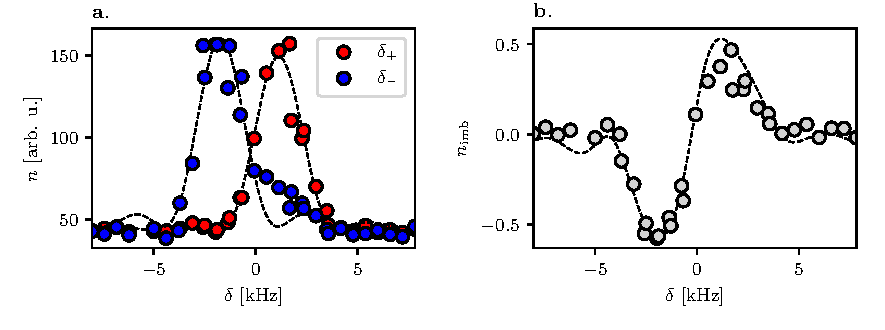
\includegraphics[]{Figures/Chapter4/uwave_lock.pdf}
\caption[Magnetic field stabilization using microwave assisted PTAI]{Magnetic field stabilization using microwave assisted PTAI. {\bf a.} Population transfered into $\ket{F=2, m_F=-1}$ from $\ket{F=1, m_f=-1}$ as a function of bias magnetic field (global detuning $\delta$). Each microwave pulse was $\tau=\unit[250]{\mu s}$ and detuned by $\delta_{\pm}=\pm 1/(2\tau)$ transfer a small fraction of atoms from $\ket{F=1, m_f=-1}$ into $\ket{F=2, m_F=-1}$. {\bf b.} Error signal calculated using the transfered atoms by each pulse. We lock the magnetic field to the $\sim\unit[5]{kHz}$ ($\unit[\sim 7]{mG}$) wide linear portion of the signal.}
\label{fig:uwave_lock}
\end{center}
\end{figure*}

In~\cite{seroka_repeated_2019} we studied partial transfer absorption imaging as minimally destructive technique for imaging ultracold atoms. See Chapter~\ref{ch:clock_states} for an alternative solution to deal with magnetic field noise. 


\section{Upgrades to the RbLi Machine}
\label{sec:RbLi_upgrades}

\subsection{Master laser system}
Previously we used a \noted{New Focus Vortex II TLB-6900} extended cavity diode laser as our master laser and a home made saturation spectroscopy setup using a Rb glass cell (see~\cite{CampbellThesis,PriceThesis}). The frequency of this laser was not very stable and the laser would constantly get out of lock. We replaced the old master laser with a \noted{Vescent photonics DBR Laser Module System} which uses a distributed Bragg reflector laser diode with no external cavity and is therefore very mechanically stable. The frequency of the laser is stabilized and controlled using the \noted{D2-210} spectroscopy module and \noted{D2-125} laser servo. The master laser system is considerably simplified as can be seen in Figure~\ref{fig:master_laser}.

\begin{figure*}[htb]
\begin{center}
\includegraphics[]{Figures/Chapter4/master_laser.pdf}
\caption[Master laser system]{Master laser system. We replaced the old Vortex II laser with a Vescent photonics DBR Laser Module System that is considerably more stable.}
\label{fig:master_laser}
\end{center}
\end{figure*}


\subsection{Raman laser system}
\label{sec:Raman_laser}

The RbLi apparatus has a laser system with wavelength close to $\unit[790]{nm}$ that is used to generate Raman induced transitions and spin-dependent potentials (see Section~\ref{sec:vector_polarizability}). The original Raman laser system consisted of a \noted{Toptica DL Pro} laser seeding a tapered amplifier mounted on a homemade copper holder. This laser system was replaced by an M squared Ti:Saphire laser (\noted{SolsTiS-400-SRX-F}) that is pumped by a $\unit[532]{nm}$ \noted{IPG GLR30} laser. We typically operate the pump laser at $\unit[14.5]{W}$, a fraction of this light is redirected into the path of a 1D optical lattice and the remaining power is used to pump the Ti:Sahpire laser. We switched to using a Ti:Saph laser because of its wide range of tunable wavelengths in the near infrared ($\unit[725-875]{nm}$) and its high power output. Figure~\ref{fig:tisaph_power} shows the typical dependence of the Ti:Saph output power as a function of pump power. 

\begin{figure*}[htb]
\begin{center}
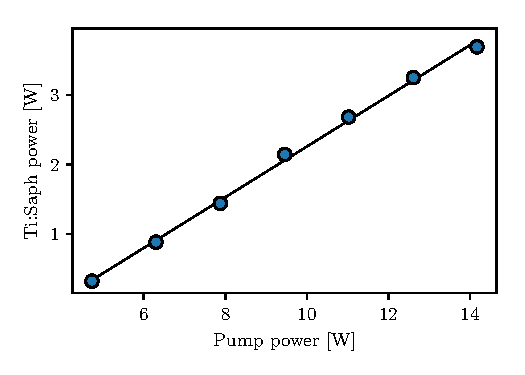
\includegraphics[]{Figures/Chapter4/tisaph_power.pdf}
\caption[Ti:Saphire laser output as a function of pump power]{Ti:Saphire laser output as a function of pump power. This data was taken when the laser was being setup for the first time. The alignment of the laser cavity was optimized to produce maximum power at $\unit[15]{W}$ pump power. The output power is proportional to the pump power $P_{\rm{out}}\approx 0.364 P_{\rm{pump}}$. }
\label{fig:tisaph_power}
\end{center}
\end{figure*}

The output of the laser is split into 3 different Raman beams. The frequency and power of each beam is independently controlled using \noted{IntraAction ATM-801A2} AOMs centered at $\unit[80]{MHz}$. We drive the AOMs using homemade drivers made from the \noted{Minicircuits} components listed in Table~\ref{table:rf_driver} and \noted{Novatech Model 409B} direct digital synthesizer (DDS) to generate an RF signal at the desired frequency. The components are arranged as is shown in Figure~\ref{fig:RF_driver}: we control the amplitude of the RF signal using a mixer connected to a DC and the switch can turn off the signal in less than $\unit[1]{\mu s}$ using a TTL signal. We fiber couple the light using single mode optical fibers (non-polarization maintaining) with FC/APC type connectors at the input  (laser side) and FC/PC at the output (experiment side). We made this choice so to implement a phase lock that would cancel phase noise added by the fibers. The idea behind this method is that a small fraction of the fiber coupled light is reflected at the flat cut edge of the optical fiber and coupled back where it can be heterodyne probed with the input light, our implementation described in Section 3.6.3 of~\cite{BeckerThesis}. We control the polarization of the light using polarization controlling paddles (\noted{Thorlabs FPC030} and \noted{Thorlabs FPC560}) which produce a controllable amount of stress in the fibers that changes their birefringence, a method that we have found to be much more stable than using polarization-maintaining fibers even when the polarization of the light is properly aligned to the fiber slow/fast axis. None of the experiments presented in this thesis used the phase lock but the experiments described in Chapter~\ref{ch:Rashba} were performed using the new Raman laser system. Figure \note{TODO: make diagram of Raman laser} shows a diagram of the Raman optics as well as the $\unit[532]{nm}$ optical lattice optics which are shared on the same breadboard. 

\begin{table}[h]
\caption[List of AOM driver components]{List of AOM driver components}
\begin{center}
\begin{tabular}{c c}
\hline
Part number & Description \\
\hline \hline
ZHL-1-2W & 2\,W amplifier \\
 ZAD-3+ & Mixer\\
 ZYSWA-2-50DR & Digital switch 
\end{tabular}
\end{center}
\label{table:rf_driver}
\end{table}

\begin{figure*}[htb]
\begin{center}
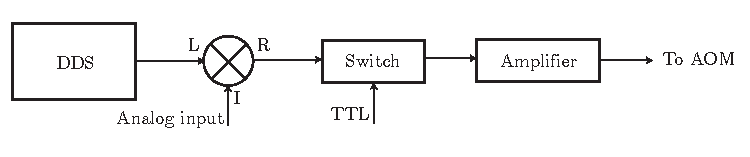
\includegraphics[]{Figures/Chapter4/RF_driver.pdf}
\caption[RF driving electronics]{RF driving electronics. We use this setup to drive the AOMs controlling the Raman beams. A similar setup is used to drive a coil used to generate high-power RF fields at the atoms (Section~\ref{sec:high_power_rf_antenna}}
\label{fig:RF_driver}
\end{center}
\end{figure*}

\subsection{High power RF system}
\label{sec:high_power_rf_antenna}

The experiments described in Chapters~\ref{ch:clock_states} and~\ref{ch:Rashba} required the use of high power RF magnetic fields to achieve coupling strengths at the atoms $\Omega\sim \unit[100-200]{kHz}$. To do so we built a resonant circuit. 
After multiple attempts to build a resonant coil either on a PCB (similar to the coil used for RF induced evaporation, see~\cite{CampbellThesis,PriceThesis}) or winding some wires with the right dimensions we found that the product that worked best for our needs was a wireless power
charging receiver coil (\noted{W\"urth Elektronik} Digikey part number \noted{732-5646-ND}) shown in the bottom panel of Figure~\ref{sec:high_power_rf_antenna}a. The coil has a self resonant frequency at $\unit[22]{MHz}$ and a Q-Factor of 45. It has an inner diameter of $\unit[1.62]{cm}$ and an outer diameter of $\unit[2.8]{cm}$, just the right side for us to place it snugly next to the glass cell (on the $-\ex$ side) with minimal perturbations to the laser beams in its vicinity (it only slightly clips one MOT beam).

\begin{figure*}[htb]
\begin{center}
\includegraphics[]{Figures/Chapter4/high_power_rf.pdf}
\caption[High power RF system]{We use a commercial resonator with an impedance matching network to produce high power RF fields. {\bf a.} Diagram of the impedance matching network. {\bf b.} A picture of the resonator mounted on a PCB. We place this device as close to the atoms as possible next to the glass cell.}
\label{fig:high_power_rf}
\end{center}
\end{figure*}

The loop is mounted on a PCB as is shown in Figure~\ref{fig:high_power_rf}. The board has two connections. The top one in Figure~\ref{fig:high_power_rf} has a small loop used as a pickup antenna that we attach to a detector \noted{Minicircuits ZX47-40-S+} to monitor the power of the antenna. The bottom lines have pads that can be used to make an impedance matching network. 

We used a vector network analyzer (VNA) to help us perform the impedance matching. The VNA sends a small amplitude frequency into the circuit and measures the amplitude and phase of the reflected power from which the impedance can be inferred. Figure~\ref{fig:impedance_matching}a shows the reflected power as a function of frequency for a test circuit and Figure~\ref{fig:impedance_matching}b shows the complex valued impedance as a function of frequency displayed on a Smith chart. The Smith chart is a helpful way to visualize the impedance of a circuit: the black circles correspond to constant resistance, with the right most point corresponding to an open circuit (infinite resistance) and the largest circle corresponding to a short circuit (zero resistance).  The arcs correspond to constant reactance; the horizontal axis corresponds to zero reactance ($\mathrm{Im}(Z)=0$), the top arcs correspond to $\mathrm{Im}(Z)>0$ and the lower arcs to $\mathrm{Im}(Z)<0$. The circuit is impedance matched when $Z=\unit[50]{Ohm}$, the standard value of RF transmission lines. We tested different components on the pads until we found a peak in reduced transmission at the desired frequency. For the particular resonant loop that we chose we found that a $\unit[10]{pF}$ capacitor soldered on the third pad and a $0\Omega$ resistor on the first pad was all we needed to get a resonant circuit near our frequency of interest $\sim\unit[23]{MHz}$. It is also important to note that it was important that the circuit was installed in its final location in the experiment when performing this tests as the other parts in the vicinity of the antenna can shift the resonant frequency. %For the particular resonant loop that we chose we found that a $\unit[10]{pF}$ capacitor soldered on the third pad and a $0\Omega$ resistor on the first pad was all we needed to get a resonant circuit near our frequency of interest $\sim\unit[23]{MHz}$. 

\begin{figure*}[htb]
\begin{center}
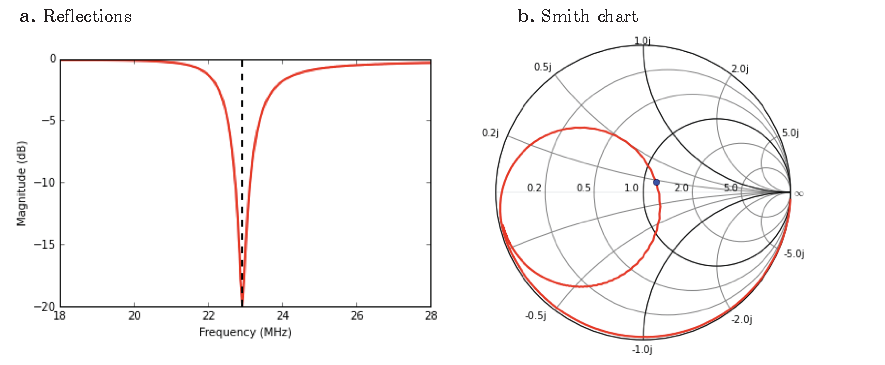
\includegraphics[]{Figures/Chapter4/impedance_matching.pdf}
\caption[Impedance matching of high power RF antenna]{Impedance matching of high power RF antenna. {\bf a.} Reflected power as a function of frequency. {\bf b.} Impedance as a function of frequency, visualized on a Smith chart. }
\label{fig:impedance_matching}
\end{center}
\end{figure*}

The driving electronics are very similar to the AOM drivers described in Section~\ref{sec:Raman_laser}. The only difference is we use a $\unit[30]{W}$ amplifier (\noted{Minicircuits LZY-22+}) instead of the smaller amplifiers needed to drive the AOMs.

\subsection{$6.8$ GHz microwave system}

Our apparatus now has a $\unit[6.8]{GHz}$ microwave system that allows us to transfer atoms between the $F=1$ and $F=2$ ground hyperfine manifolds of $\Rb87$. We mostly use this system to stabilize the bias magnetic field along $\ez$ at the atoms using microwave assisted partial transfer absorption imaging (PTAI) (see~\ref{sec:ptai}). A list of components used to in the setup is presented in Table~\ref{table:microwave_electronics} and a diagram of the connections is displayed in Figure xxx.

 \begin{table}[h]
\caption[$6.8$ GHz microwave system components]{$6.8$ GHz microwave system components}
\begin{center}
\begin{tabular}{ll}
\hline
Part number & Description \\
\hline \hline
SRS SG384 & Signal generator \\
Narda 4014C-30 & Directional coupler\\
Marki IRW0618  & Mixer \\
Minicircuits VBFZ-6260-S+ & Bandpass filter $\unit[6-8]{GHz}$ \\
Herley D1956 & Voltage controlled attenuator \\
MSI MSH-5727901  & $\unit[46]{dB}$ gain amplifier \\
Narda 4014C-30 & Circulator \\
Minicircuits ZX47-40-S+ & Power detector \\
Maury microwave 1819C & Stub tuner \\
 ZYSWA-2-50DR & Digital switch \\
\hline \hline
\end{tabular}
\end{center}
\label{table:microwave_electronics}
\end{table}
%
The SRS generator serves as a source of a fixed frequency and amplitude signal. We control the frequency by mixing a programmable $\sim \unit[100]{MHz}$ signal from a \noted{Novatech} into a double balanced mixer; the RF signal can be turned on or off using a TTL switch. The amplitude is controlled by commanding $\unit[0-6]{V}$ signal from the control computer into an attenuator. The signal is amplified by $\unit[+43]{dB}$ using an amplifier mounted on a water cooled plate. The microwave signal is broadcast to the atoms using a horn antenna. The impedance of the transmission line is tuned with the a stub tuner such that reflections are minimized. We additionally use a circulator that prevents any reflected power to go back into the amplifier. We use couplers at different locations to monitor the performance of the system.  

\section{Computer control and data acquisition}

There have been two main changes in our computer control and data acquisition system. We have transitioned from using a \noted{LabVIEW} based control system to a Python based control system \noted{The labscript suite}~\cite{starkey_scripted_2013}. In the previous control software the lab devices were programmed using a graphic interface. \noted{Labscript} instead uses a hybrid approach in which the experimental sequences are based text scripts. The use of scripted programming makes our experiments very modular and additionally it is now very easy to do multi-dimensional parameter scans, both things that were not straightforward to do in the past. Each experimental shot is saved in a Hierarchical Data Format version 5 file (HDF5). The file includes images from cameras, oscilloscope traces and analog inputs as well as copy of the script used in the experiment and the values of the parameters used. This has been a great upgrade as we no longer rely on the person running an experimental sequence pushing the `save' button and fully documenting the experiment in question\footnote{As I have been digging into old data, I greatly wish we had this feature sooner}. 

The other upgrade worth mentioning is replacing our old \noted{Flea3} CCD camera with a \noted{Mako G-030} camera from \noted{Allied Vision}. With this new camera the time between two consecutive shots can be as small as $\unit[96]{\mu s}$ (used to be $\sim\unit[15]{ms}$ with the Flea3 camera), greatly reducing the effect of mechanical vibrations in the experiment that produce fringes in the absorption images. The addition of this camera was essential to get a better signal to noise ratio in the experiments reported in Chapter~\ref{ch:Rashba}. Figure \note{TODO: make before and after Mako figure} shows and absorption image of thermal atoms taken with the old flea 3 and the...

%Figure~\ref{fig:labscript} shows an experimental sequence where a BEC is made using the steps described in Section~\ref{sec:making-becs} and an absorption image is taken at the end. We typically separate th

% \begin{figure*}[htb]
% \begin{center}
% 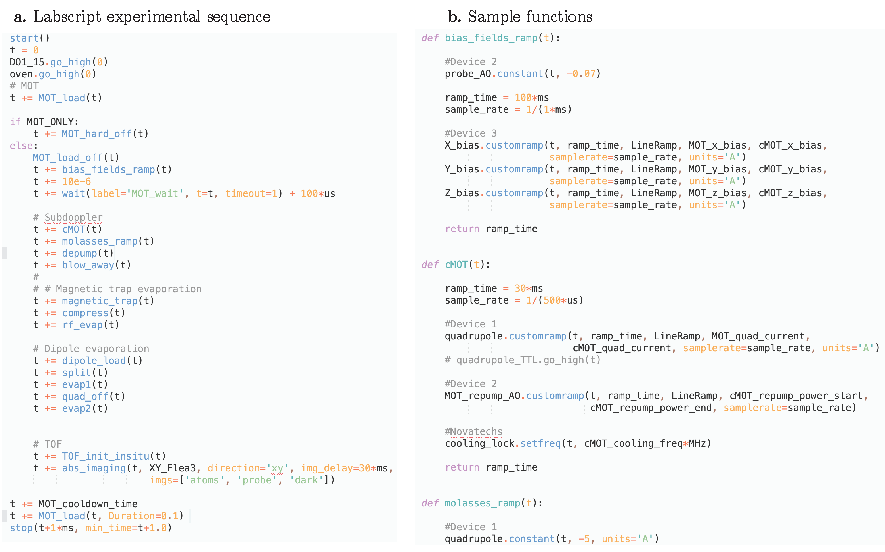
\includegraphics[]{Figures/Chapter4/labscript.pdf}
% \caption[Impedance matching of high power RF antenna]{Impedance matching of high power RF antenna}
% \label{fig:labscript}
% \end{center}
% \end{figure*}


% We then apply a pair of $250\,\mu\mathrm{s}$ microwave  pulses that each transfer a small fraction of atoms into the $5^2{\rm S}_{1/2}$ $f=2$ manifold that we use to monitor and stabilize the bias field \cite{leblanc_direct_2013}. The microwave pulses are detuned by $\pm 2\, \kHz$ from the $\ket{f=1,m_F=0}\leftrightarrow\ket{f=2,m_F=1}$ transition and spaced in time by $33\, \mathrm{ms}$ (two periods of $60\, \mathrm{Hz}$). We imaged the transferred atoms following each pulse using absorption imaging\footnote{We did not apply repump light during this imaging, so the untransferred atoms in the $f=1$ manifold were largely undisturbed by the imaging process.}, and count the total number of atoms $n_1$ and $n_2$ transferred by each pulse. The imbalance in these atom numbers $(n_1-n_2)/(n_1+n_2)$ leads to a $4\kHz$ wide error signal that we use both to monitor the magnetic field before each spectroscopy measurement and cancel longterm drifts in the field. 

